\chapter{Implementation}
\label{sec:implementation}
\index{CRAVA!implementation}

Whereas the general model was explained in \autoref{sec:theory} we explain a bit more of the actual implementation details here.

\section{Using FFT for inversion}
As previously stated, \autoref{eq:WADm} separates when transformed into the Fourier domain. After this transformation, the equation becomes
\begin{equation}
\label{eq:fourierinv}
\vect{\tilde{d}}(\omega,\vect{k}) = \vect{G}(\omega)\vect{\tilde{m}}(\omega,\vect{k}) + \vect{\tilde{e}}(\omega,\vect{k}))
\end{equation}
The $\tilde{ }$ denotes the 3D fourier transform, with temporal frequency $\omega$, and lateral frequency vector $\vect{k} = (k_x,k_y)$. Due to the separation, we now have a set of $n$ small equations, where $n$ is the number of grid cells in the inversion volume. Everything is still normally distributed, so the solution to this equation follows the pattern from \autoref{eq:mupost} and \autoref{eq:sigmapost}. We still must invert a data covariance matrix, but whereas this matrix had dimension $(n\cdot n_\theta)^2$ before the Fourier-transform, the matrix we must invert here is reduced to dimension $n_\theta^2$, where $n_\theta$ is the number of angle stacks. Since the time for a matrix inversion is almost cubic in size, it is much faster to invert $n$ of these small matrixes than the one large. After solving for $\vect{\tilde{m}}(\omega,\vect{k})$, we do the inverse transform of this to obtain the distribution for $\vect{m}$. The same does of course hold when we are using local wavelets that are divided out in advance, \autoref{eq:ADm}. For full details, see \cite{geo68ab2}.

\section{Local wavelet and noise}
\label{sec:nonstationaryimp}
As shown, even though the use of FFT-transform requires stationarity,
we are able to work around this. Wavelets can be made local since
these can be divided out before solving the problem, and locally
higher noise levels can be approximated by interpolating the low-noise
solution and the prior distribution. 

\subsection{Dividing out the wavelet}
\label{sec:divwavimp}
A simple division of data by wavelet can easily be done in the Fourier domain, since the convolusion there is reduced to a multiplication, and the division can be done one frequency at a time. However, this is very unstable for frequencies where the wavelet is very weak or not present, so some stabilizing is needed.

In \crava this is done in two ways. First, we set an upper and lower cutoff frequency for the wavelet, default set to 5 and 55 Hz. Furthermore, for frequencies that fall below 10\% of the average amplitude, we set the amplitude to 10\% of average before doing the division.

\subsection{Local noise}
\label{sec:localnoiseimp}
Local noise is implemented by first finding the solution using the minimum noise level, to fulfill the stationarity requirements of the FFT algorithm. We then interpolate the values for each locations between the prior and this minimum noise posterior. When doing this interpolation, we ignore correlation between locations. This is not a problem as long as the noise varies slowly and smoothly.


For each location $\vect{x}$ the adjusted estimate $\tilde{\bmu}_{m|d_{obs}}(\vect{x})$, is found
from the inversion result $\bmu_{m|d_{obs}}(\vect{x})$ by a linear relation,
\begin{equation} \label{eq:LocalAdjustment}
\tilde{\bmu}_{m|d_{obs}}(\vect{x}) = \bmu_{m}(\vect{x}) +\vect{H_x}\left(\bmu_{m|d_{obs}}(\vect{x})-\bmu_{m}(\vect{x})\right),
\end{equation}
The matrix $\vect{H_x}$ is a shrinkage matrix, i.e. the adjusted estimate
is always closer to the prior mean than the inversion result. The matrix
$\vect{H_x}$ depends on the local error variance
 $\bSigma_{e}^x$ and error variance used in the inversion $\bSigma_{e}^0$.

To find the shrinkage matrix we first identify a matrix $\vect{G}_0$
which is such that it maps the local prior distribution to the local posterior distribution
when it is observed with the noise $\Sigma_{e}^0$, i.e.
$$ \vect{d}(\vect{x}) = \vect{G}_0\vect{m}(\vect{x})+\vect{e}_0,$$
where $\vect{e}_0\sim N\left( \vect{0},\Sigma_{e}^0\right)$.
The inversion of this expression is a linear relation
 \begin{equation} \label{eq:PSigmae}
\bmu_{m|d_{obs}} =\bmu_{m} +\vect{P}(\Sigma_{e}^0)\left(\vect{d}_{obs}-\bmu_{d}\right)
\end{equation}
where  $\vect{P}(\Sigma_{e}^0)=\bSigma_{m}\vect{G}_0^T \left( \vect{G}_0\bSigma_{m}\vect{G_0}^T+\bSigma_{e}^0\right)^{-1}$.

We then define the shrinkage matrix to be:
\begin{equation}\label{eq:H}
\vect{H_x}(\Sigma_{e}^\vect{x},\Sigma_{e}^0) = \vect{P}(\Sigma_{e}^\vect{x})\vect{P}(\Sigma_{e}^0)^{-1}.
\end{equation}
By this we mean that we remove the effect of the standard inversion and add the effect of
the locally adapted inversion. The matrix $\vect{P}(\Sigma_{e}^0)$ is not invertible,
but since the local noise always is larger than the noise in the inversion the product in
expression $\ref{eq:H}$ is always well defined.


\section{Estimation of parameters}
\label{sec:estimateimp}
The estimation routines implemented in \crava are based on straightforward and commonly used techniques. This gives fast and robust estimation, although we may run into problems if the number of data points is too small, or the data quality is too low. The quality of an estimation result is never better than the quality of the data it is based on.
\subsection{Estimating wavelet and noise}
\label{sec:waveestimp}
The wavelet estimation in \crava is based on \cite{White84}. Wavelets are estimated at well locations, where we obtain the reflection coefficients from well logs. We then use the relation
\begin{equation}
\vect{d} = \vect{w}*\vect{c}+\vect{e}
\end{equation}
where $\vect{d}$ is the seismic amplitude data, $\vect{w}$ is the wavelet, $\vect{c}$ the reflection coefficients, and $\vect{e}$ is the noise. We transform this to the Fourier domain, multiply with with the reflection coefficients, and take the expectation to get
\begin{equation}
d(\omega)\bar{c}(\omega) = w(\omega)|c(\omega)|^2
\end{equation}
Note that the convolution has disappeared, and the equation can be solved for each frequency $\omega$. However, solving this directly in the frequency domain is unstable, so we need to do a frequency smoothing. This is done by transforming $d(\omega)\bar{c}(\omega)$ and $|c(\omega)|^2$ back to time domain, multiplying with a Papoulis taper, and transforming them back to the frequency domain. This is the same as applying a local smoothing in the frequency domain. After this, we divide out $w(\omega)$, and transform back to time domain.

We find the optimal vertical shift for each well. The global wavelet is then found by taking the arithmetic average of the zero-phase wavelets, weighted by the number of samples used from each well. The noise estimate is found by generating synthetic seismic using the averaged wavelet optimally shifted in each well, and subtracting this from the seismic data. The remaining part is assumed to be noise, and we measure the noise energy from this.

When using local wavelets, we find the optimal shift and/or scale of
the global wavelet at each well location. Optimal here means
minimizing the noise energy. We then use kriging to interpolate this
between wells, with a shift of 0 and a scale of 1 as the mean level
outside the well control area.  This is illustrated in
\autoref{fig:local-wavelet}. 

\begin{figure}
  \centering
  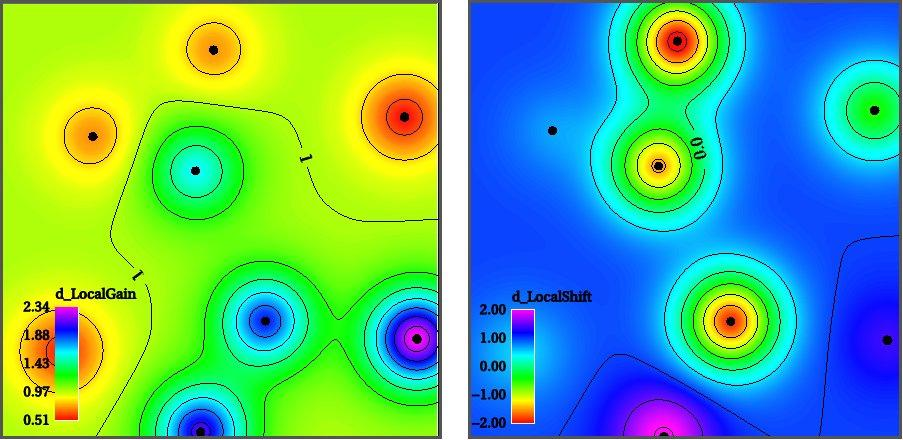
\includegraphics[width=.95\linewidth]{images/local-wavelet}
  \caption{The local scale and shift maps involved when using local wavelets}
  \label{fig:local-wavelet}
\end{figure}

Local noise is estimated using the local noise energies from above. We always use local shift when estimating the noise, but only use local scale if it is used in the inversion. If local scale is used, the noise is divided by this. A noise scaling factor is then computed in each well, and kriged as above.

\subsection{Estimating 3D wavelet}
\label{sec:3Dwaveestimp}
The expression for the 3D wavelet given in \autoref{eq:waveletform} has only one unknown element, namely the 1D pulse $w_0(\omega)$. As for the 1D wavelet, the pulse is estimated from wells. Using reflection coefficients from well logs, time gradients estimated from seismic around wells and depth gradients computed from time gradients by using reference time surface and average velocity given by the user, a linear regression model can be set up for the seismic as
\begin{equation}
\vect{d} = \vect{K}\vect{w}_0 + \vect{e}.
\end{equation}
The least squares estimate for $\vect{w}_0$ is
\begin{equation}
\widehat{w}_0 = (\vect{K}'\vect{K})^{-1}\vect{G}'\vect{d}.
\end{equation}

\subsection{Estimating correlations}
\label{sec:correstimp}
We estimate correlations by first blocking the wells into the grid, and then do standard correlation estimation using
\begin{equation}
\text{Cov}(X,Y) = \text{E}(XY)-E(X)E(Y).
\end{equation}
Since we model the covariance structure as separable, we have to collapse the full time dependent covariances between parameters into one parameter covariance matrix and a temporal correlation vector. This is done simply by using the covariances at time lag 0 as our covariance matrix, and averaging the remaining time correlation vectors for the parameters.

\subsection{Estimating background model}
As with the correlation estimation, the first step is to block the wells into the modeling grid. We then filter away everything above a cutoff frequency (default 6Hz) from the well logs. The next step is to take the average of all log data in each grid layer, giving a vertical trend. This trend is then smoothed using a moving average smoother, and finally filtered with the cutoff frequency. We then use kriging of the well logs with this vertical trend as expectation to create the final background model.

\subsection{Estimating optimal well location}
The positioning uncertainty between well data and seismic data is often significant. To overcome this, the well may be moved to the location with maximum correlation between the seismic data and the reflection coefficients calculated from the well data. The relation between the seismic data and reflection coefficients is linear; so linear covariance is a good measure. The optimial well location is found by searching for the location with highest covariance in a lateral neighborhood around the original well location, where the well is allowed to be shifted vertically in each target position. The moving of wells is triggered by a command in the model file, and it is done prior to the estimation of wavelets, noise, correlations and background model.

\section{Memory handling}
The memory handling in \crava will primarily use memory to achieve speed. However, since the involved grids can be very large, we try to economize with the number of grids kept in memory. We also have a secondary option where we store more on disk, which will reduce memory use with a factor of at least 2 in realistic cases, but will also increase the running time by a factor of almost 3. We have both padded and unpadded grids. We count and check the number of padded grids used in detail, unpadded grids are only counted in memory computations. In the following, any mention of grid means padded, unpadded will be explcitly stated. Padded grids require $s_p$ MB memory, unpadded $s_u$.

\subsection{Grid allocation with all grids in memory}
 If the file option is not used, the grid memory allocation will go as follows:

\begin{enumerate}
\item Background grids for Vp, Vs and density, 3 grids.
\item If these are estimated, another 3 grids are allocated for estimation, but destroyed before any other allocations.
\item Seismic grids, $n_\theta$. If well optimisation is used, this will come before background grids.
\item Possibly prior facies probability grids, indicated by $I_p$, $n_f$ unpadded grids.
\item Prior covariance, 6 grids.
\item If relative facies probabilities or local noise, a copy of background indicated by $I_b$, 3 grids.
\item {\bf Peak:} At this stage, \crava reaches its first memory peak. Minimum memory use 10 grids, typical situation with three seismic grids and facies modelling requires 15 grids. \\ 
    Memory use: $P_1 = (9+n_\theta+I_b*3)*s_p+I_p*n_f*s_u$.
\item The posterior distribution is computed into the background and prior covariance grids, and seismic residuals are computed into the seismic grids. Thus, the inversion requires no extra grids. (But we needed a copy of the background for local noise or facies.)
\item After the inversion, the seismic grids are released, taking us off peak down to a base level: \\ Memory use: $(9+I_b*3)*s_p+I_p*n_f*s_u$.
\item If simulation is used:
\begin{enumerate}
\item Simulated grids are allocated, 3 grids.
\item If secondary parameters are used, indicated by $I_s$, a computation grid is allocated, 1 grid.
\item If kriging is used, indicated by $I_k$, 1 unpadded grid, not concurrent with computation grid. 
\end{enumerate}
\item {\bf Peak:} New possible peak, since the number of grids now allocated may be larger than the released seismic grids. \\
    Memory use: $P_2 = s_p*(12+I_b*3+I_s)+(I_p*n_f + max(0,I_k-I_s))*s_u$.
\item New release of grids, back to $s_p*(9+I_b*3)+I_p*3*s_u$.
\item If facies probabilities:
\begin{enumerate}
\item 3D histograms of elastic parameters per facies are created, each of size 2MB, $n_f$ special grids.
\item Facies probability grids are created, including for undefined, $n_f+1$ unpadded grids.
\end{enumerate}
\item {\bf Peak:} New possible peak, since the new memory allocated may be larger than the released seismic grids and/or the simulation+computation/kriging grids. \\
    Memory use: $P_3 = (9+I_b*3)*s_p+(I_p*n_f + n_f +1)*s_u + 2*n_f$.
\item Can now release all grids related to facies probability, memory down to $s_p*9$.
\item Eventual kriging of prediction allocates 1 unpadded grid.
\item Everything released.
\end{enumerate}

The maximum memory use is thus the largest of the actual peaks. The maximum number of allocated padded grids will occur at either $P_1$ or $P_2$, whereas the largest number of other grids are allocated at $P_3$. 
